%%%%%%%%%%%%%%%%%%%%%%%%%
% Dokumentinformationen %
%%%%%%%%%%%%%%%%%%%%%%%%%
\newcommand{\titleinfo}{OOAD - Formelsammlung}
\newcommand{\authorinfo}{J\"urg \& DIE Schweisser}
\newcommand{\versioninfo}{$Revision: 1 $}  

%%%%%%%%%%%%%%%%%%%%%%%%%%%%%%%%%%%%%%%%%%%%%
% Standard projektübergreifender Header für
% - Makros 
% - Farben
% - Mathematische Operatoren
%
% DORT NUR ERGÄNZEN, NICHTS LÖSCHEN\newpage
%%%%%%%%%%%%%%%%%%%%%%%%%%%%%%%%%%%%%%%%%%%%%
\include{header/header}
\usepackage{listings}
%\usepackage{textcomp}
\definecolor{lbcolor}{rgb}{0.92,0.92,0.92}
\lstset{
	backgroundcolor=\color{lbcolor},
	tabsize=4,
	rulecolor=,
	language=c++,
    basicstyle=\scriptsize,
    upquote=true,
        aboveskip={0.5\baselineskip},
        columns=fixed,
        showstringspaces=false,
        extendedchars=true,
        breaklines=true,
        prebreak = \raisebox{0ex}[0ex][0ex]{\ensuremath{\hookleftarrow}},
        frame=single,
        showtabs=false,
        showspaces=false,
        showstringspaces=false,
        identifierstyle=\bfseries\ttfamily,
        keywordstyle=\color[rgb]{0,0,1},
        commentstyle=\color[rgb]{0.133,0.545,0.133},
        stringstyle=\color[rgb]{0.627,0.126,0.941},
}

\begin{document}
\section{C++ CheatSheet}

\subsection{Header Files}
\begin{multicols}{2}
	\textbf{Include-Guard:}
	\begin{lstlisting}
	#ifndef MeinHeader_H
	#define MeinHeader_H
	// Ganzer Inhalt vom Header
	#endif
	\end{lstlisting}
	
	\textbf{Header und using namespace:} \\
	Kein \lstinline!using namespace std;! Wenn eine Funktion aus
	dem diesem Namespace gebraucht wird kann mit dem vollen Namen darauf
	zugegriffen werden. (\lstinline!std::cout << "..." << std::endl;!)
\end{multicols}


\subsection{Unterschied Statisch - Dynamisch}
\begin{multicols}{2}
\textbf{Statisch:}
\begin{lstlisting}
ClassA a;
a.foo(); // Funktionsaufruf
bar(&a); // Uebergabe von this
\end{lstlisting}

\textbf{Dynamisch:} 
\begin{lstlisting}
ClassA* a = new A();
a->foo(); // Funktionsaufruf
bar(a); // Uebergabe von this
\end{lstlisting}
\end{multicols}

\subsection{Assoziationen}
\subsubsection{"`0..1:0..1"'}
\begin{multicols}{2}
Vorwärtsdekleration wird gebraucht, wenn zwei Klassen sich gegenseitig referenzieren. \\

\textbf{Header A:}
\begin{lstlisting}
class B; // Vorwaertsdeklaration

class A{
	public:
	    A();
		void setB(B* pB);
		B* getB();
		
	private:
		B* mB; // Pointer auf B-Objekt
};
\end{lstlisting}

\textbf{Implementation:}
\begin{lstlisting}
void A::setB(B* pB) {
	mB = pB;
}
\end{lstlisting}

\columnbreak
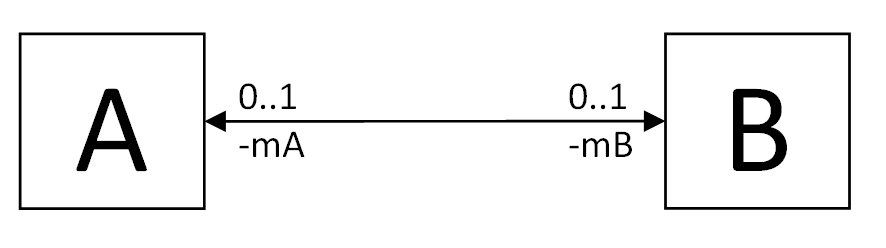
\includegraphics[width=5cm]{./bilder/Assozi_01_01.png}

\textbf{Header B:}
\begin{lstlisting}
class A; // Vorwaertsdeklaration

class B {	
	public:
		B();
		void setA(A* pA);
		A* getA();
		
	private: 
		A* mA; // Pointer auf A-Objekt
};
\end{lstlisting}

\textbf{Aufruf:}
\begin{lstlisting}
A a;
B b;
a.setB(&b);
\end{lstlisting}
\end{multicols}

\subsubsection{"`1:0..1"'}
Eine 1:0..1 Assoziation kann ähnlich wie eine 0..1:0..1 Assoziation
implementiert weden. Wobei auf der "`1 Seite"' die andere Klasse direkt im
Konstruktor mitgegeben wird. Ein Setter wird auf der B-Seite nicht mehr
gebraucht! Achtung: untenstehende Implementation zeigt nur schematisch auf wie
es funktioniert. Copy- und Zuweisungskonstruktor müssten auch noch korrekt
implementiert werden.
\begin{multicols}{2}
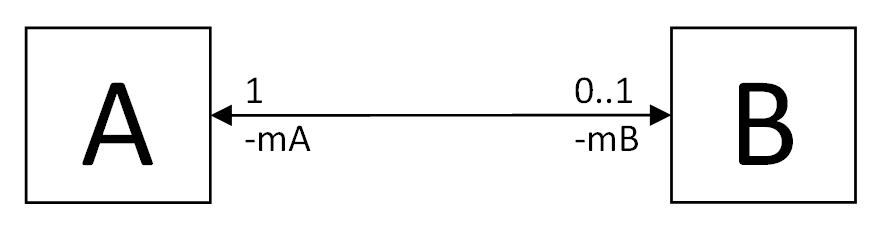
\includegraphics[width=5cm]{./bilder/Assozi_1_01.png}\\
\textbf{Header B (Muss Assoziation)}
\begin{lstlisting}
// ...
class B {
	public: 
		A* getA();
		B(A* pa);		// Konstruktor
	
	private:
		A* mA;		
		B();			// Default Konstruktor
}
\end{lstlisting}
\columnbreak
\textbf{Implementation B (Muss Assoziation)}
\begin{lstlisting}
B::B(A* pA)
: mA(pA)
{
	mA->setB(this); 
	// Kann auch im im Aufruf erfolgen
}
\end{lstlisting}

\textbf{Aufruf:}
\begin{lstlisting}
	A a;
	B b(&a);
\end{lstlisting}
\end{multicols}

\newpage

\subsubsection{"`0..1:0..n"'}
\begin{multicols}{2}
\textbf{Header A:}
\begin{lstlisting}
class B; // Vorwaertsdeklaration

class A{
	private:
		B* mB[n]; // Pointerarray auf B-Objekte
	
	public:
	    A();
		void addB(B* pB);
		void removeB(B* pB);
};
\end{lstlisting}

\textbf{Implementation:}
\begin{lstlisting}
A::A() {
	for(int i = 0; i<n; i++) {
		// Alle Werte auf 0 initialisieren
		mB[i] = 0; 
	}
}

// fuer removeB sinngemaess (->setA(0); mB[i]=0)
void A::addB(B* pB) {
	for(int i = 0; i<n; i++) {
		if(mB[i] == 0) {
			mB[i] = pB;
			mB[i]->setA(this);
			return;
		}
	}
}
\end{lstlisting}

\columnbreak
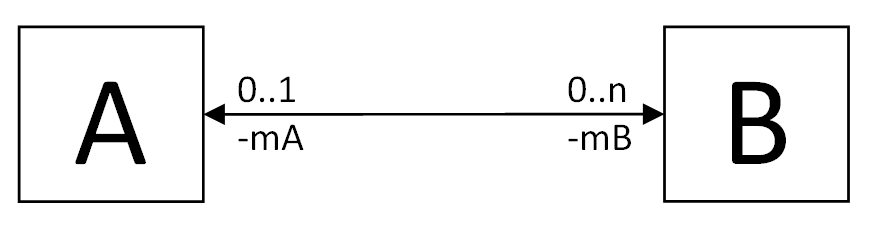
\includegraphics[width=5cm]{./bilder/Assozi_01_0n.png}\\
\textbf{Header B:}
\begin{lstlisting}
class A; // Vorwaertsdeklaration

class B {
	private: 
		A* mA; // Pointer auf A-Objekt
		
	public:
		B();
		void setA(A* pA);
		A* getA();
};
\end{lstlisting}

\textbf{Aufruf:}
\begin{lstlisting}
A a;
B b1;
B b2;
a.addB(&b1);
a.addB(&b2);
a.removeB(&b2);
// ...
\end{lstlisting}
\end{multicols}

\subsection{Vererbung}
\begin{multicols}{2}
\textbf{Basisklasse}
\begin{lstlisting}
	class: Fahrzeug
	{
	public:
			 Fahrzeug(int pGewicht);
		void setGewicht(int pGewicht);
	
	private:
		int mGewicht;
	};
\end{lstlisting}

\columnbreak

\textbf{abgeleitete Klasse}
\begin{lstlisting}
	class: Auto : public Fahrzeug
	{
	public:
			 Auto(int pPersonen, int pGewicht);	
		void setPersonen(int pPersonen);
		
	private:
		int	mPersonen;
	}	
\end{lstlisting}
\end{multicols}

\textbf{Aufruf}
\begin{lstlisting}
	Auto.setGewicht(42);
	Auto.setPersonen(4);
\end{lstlisting}





\section{Begriffe}
\subsection{Klasse}
	Eine Klasse ist eine Vorlage für ein Objekt.\\
	\begin{description}[style=multiline,leftmargin=3.5cm,rightmargin=2cm, topsep=0pt]
	\item[Attribut] Beschreibt Daten die von den Objekten der Klasse angenommen
		werden können. Alle Objekte einer Klasse haben dieselben Attribute, können
		aber unterschiedliche Attributwerte haben.
	\item[Klassenattribut] wenn nur ein Attributwert für alle Objekte einer Klasse
		existiert. Sie existieren auch, wenn es zu einer Klasse noch keine Objekte
		gibt.
	\item[Operation] Eine Funktion die auf alle Attributwere eines Objekts Zugriff
		hat.
	\item[Klassenoperation] Eine Operation, die der jeweiligen Klasse zugeordnet
		ist kann nicht auf ein einzelnes Objekt der Klasse angewendet werden. 
	\item[Verhalten] Das Verhlaten der Klasse ist die Menge aller Operationen
	\item[Abstrakte] Von einer abstrakten Klasse können keine Objekte erzeugt
		werden.
	\item[Basisklasse] Vererbt abgeleiteten Klassen Attribute und Operationen
	\end{description}
	
\subsection{Objekt}
	Ein Objekt wird aus einer Klasse erzeugt, ist also ein Exemplar einer Klasse.
	\begin{description}[style=multiline,leftmargin=3.5cm,rightmargin=2cm, topsep=0pt]
		\item[Zustand] bestimmt durch seine Attributwerte und seine
		Objektbeziehungen zu anderen Objekten
		\item[Verhalten (behavior)] die beobachtbaren Effekte aller Operationen
		 bestimmt durch die Operationsaufrufe, auf die diese Klasse bzw. deren Objekte
		reagieren.
		\item[Objektidendität] jedes Objekt besitzt eine, sind unique
	\end{description}
\subsection{Komponente}
Ist ein Softwarebaustein, der über klar definierte Schnittstellen Verhalten
(Funktionalität) bereitstellt.
interface
component

\subsection{Assoziation}
	modelliert Objektbeziehungen zwischen Objekten einer oder mehrerer Klassen. Jede
	Assoziation wird durch Mutliplizitäten, einen optionalen Namen oder Rollennamen
	beschrieben.\\
	\begin{description}[style=multiline,leftmargin=3.5cm,rightmargin=2cm, topsep=0pt]
		\item[ternäre Assoziation] Assoziation zwischen 3 Objekten.
		\item[n-äre Assoziation] zwischen n Objekten
		\item[reflexive Assoziation ] verbindet zwei Objekte einer Klasse
		\item[binäre Assoziation] verbindet zwei Objekte 
		\item[Assoziationsklasse] besitzt die Eigenschaften einer Assoziation und
		einer Klasse 
		\item[Aggregation] Sonderfall der Ass. "`ist Teil von"' oder "`besteht
		aus"'.
		\item[Komposition] besondere Form der Aggregation. Beim Löschen müssen auch
		alle Teile gelöscht werden. Jedes Teil kann nur zu einem Ganzen gehören.
		\item[Navigationsrichtung] das erzeugen des einen erzwingt die Erzeugung des
		anderen
		\item[Multiplizität] bezeichnet die Wichtigkeit der Assoziation. Bezeichnet
		die Anzahl der an der Assoziation beteiligten Objekte.
		\item[abgeleitete Assoziation]
		die Abhängigkeiten sind bereits durch andere Assoziationen beschrieben worden
		\item[Assoziationname] beschreibt im Allgemeinen nur eine Richtung der
		Assoziation. kann fehlen wenn captain obvious unterwegs ist
		\item[Leserichtung] angabe beim Assoziationsnamen
		\item[Sichtbarkeit] Vor den Rollennamen geschrieben. -private \#protected
		+public $\sim$ package
		\item[Eigenschaftswert] kann bei Bedarf ans Assoziationsende geschrieben
		werden. Ordnend.
		\item[Rollenname] bei der Klasse, deren Bedeutung sie beschreibt. Kann zur
		verständlichkeit Beitragen
	\end{description}

\subsection{Generalisierung}
Beschreibt die Beziehung zwischen einer allgemeinen Klasse (Basisklasse) und
einer spezialisierten Klasse. Die spezialisierte Klasse ist vollständig
konstistent mit der Basisklasse, enthält aber zusätzliche Informationen
(Attribute, Operationen, Assoziationen).
	\begin{description}[style=multiline,leftmargin=3.5cm,rightmargin=2cm, topsep=0pt]
		\item[Vererbung] Unterklasse kann alle eigenschaften als Oberklasse
		mitbenutzen
		\item[Einfachvererbung]
		\item[Mehrfachvererbung]
		\item[Generalisierung] Die spezialisierte Klasse erweitert die Liste der
		Attribute, Operationen und Assoziationen der Basisklasse
		\item[Generalisierungsmenge] spezifiziert, nach welchen Kriterien eine
		Generalisierung modelliert wird
	\end{description}
	
\subsection{Use-Case Diagramm}
	Ein Use-Case spezifiziert eine Sequenz von Aktionen
	\begin{description}[style=multiline,leftmargin=3.5cm,rightmargin=2cm, topsep=0pt]
		\item[Akteur] ist eine Rolle, die ein Benutzer des Systems spielt. Jeder
		Akteur hat einen Einfluss uaf das System. Befindet sich stets ausserhalb des Systems\\
	\end{description}

\end{document}
